\documentclass{article}

\usepackage[final]{neurips_2026}

\usepackage[utf8]{inputenc}
\usepackage[T1]{fontenc}
\usepackage{hyperref}
\usepackage{url}
\usepackage{booktabs}
\usepackage{amsmath}
\usepackage{amsfonts}
\usepackage{amssymb}
\usepackage{graphicx}
\usepackage{xcolor}
\usepackage{microtype}

\title{Edge-Gated Self-Play PPO for a Unity-Based Sumo Arena}

\author{%
  Julie Yang\\
  Deep Reinforcement Learning Course Project\\
  \texttt{sumo-selfplay-rl}\\
}

\begin{document}

\maketitle

\begin{abstract}
This report presents a compact Unity-based self-play reinforcement learning system for a two-agent sumo-style arena. Two circular agents move in a bounded 2D physics environment and attempt to push each other out of a circular ring. The project combines a Unity simulation, a TCP bridge, Python environment wrappers, trajectory collection, checkpoint evaluation, imitation learning utilities, and PPO-based self-play training. Beyond a plain PPO baseline, the implementation explores several lightweight stabilization strategies: alternating two-policy self-play, opponent-pool sampling, Gaussian policy mutation, exponential moving average propagation, reward and observation shaping, and a proposed Edge-Gated Actor-Critic (EGAC). EGAC injects arena-specific boundary risk into the actor by damping outward movement and reducing push probability near the arena edge. The main contribution is an end-to-end experimental platform and a structured method for studying brittle boundary behavior in physical self-play environments.
\end{abstract}

\section{Introduction}

Self-play is a natural training mechanism for symmetric competitive tasks. It removes the need for a fixed expert opponent and can produce curricula automatically as agents improve against earlier versions of themselves. However, self-play also introduces familiar difficulties: the opponent distribution is non-stationary, policies can overfit to the latest opponent, and seemingly improving agents can collapse into brittle behaviors. These issues are especially visible in simple physical games where a small action error can immediately produce a terminal failure.

This project studies those issues in a small Unity-based sumo arena. Two circular agents are placed in a 2D circular ring. Each agent can move continuously and trigger a push or dash action with a cooldown. A match ends when one agent leaves the playable boundary or when a time limit is reached. Although the rules are intentionally minimal, the environment exposes several common multi-agent reinforcement learning problems. Agents may learn to overuse push, drift toward the edge, exploit only the current opponent, or lose by self ring-out. These failure modes are easy to inspect visually, which makes the environment useful for a course project focused on both learning and demonstration.

The project began as an end-to-end systems challenge: connecting Unity physics to Python training code, defining a compact observation space, collecting rollouts, saving checkpoints, and evaluating policies back inside Unity. After this pipeline became operational, the main challenge shifted toward stabilizing self-play and reducing degenerate behavior. A plain PPO actor-critic provides the base learning algorithm, while the final implementation adds a sequence of self-play extensions and an arena-specific network modification.

The contributions of the project are:
\begin{enumerate}
    \item A Unity-driven two-agent sumo environment with a Python TCP bridge, batched arena stepping, and human-vs-policy demonstration support.
    \item A PPO training stack supporting rollout collection, checkpointing, vectorized observations, and alternating two-policy self-play.
    \item A set of lightweight self-play stabilization mechanisms: opponent-pool sampling, Gaussian policy mutation, exponential moving average propagation, and reward/observation shaping.
    \item Edge-Gated Actor-Critic (EGAC), a boundary-aware actor architecture that uses edge-margin features to reduce outward movement and risky push actions near the ring boundary.
    \item An ablation protocol and qualitative analysis plan for comparing plain PPO, alternating self-play, enhanced self-play, and EGAC.
\end{enumerate}

\begin{figure}[t]
    \centering
    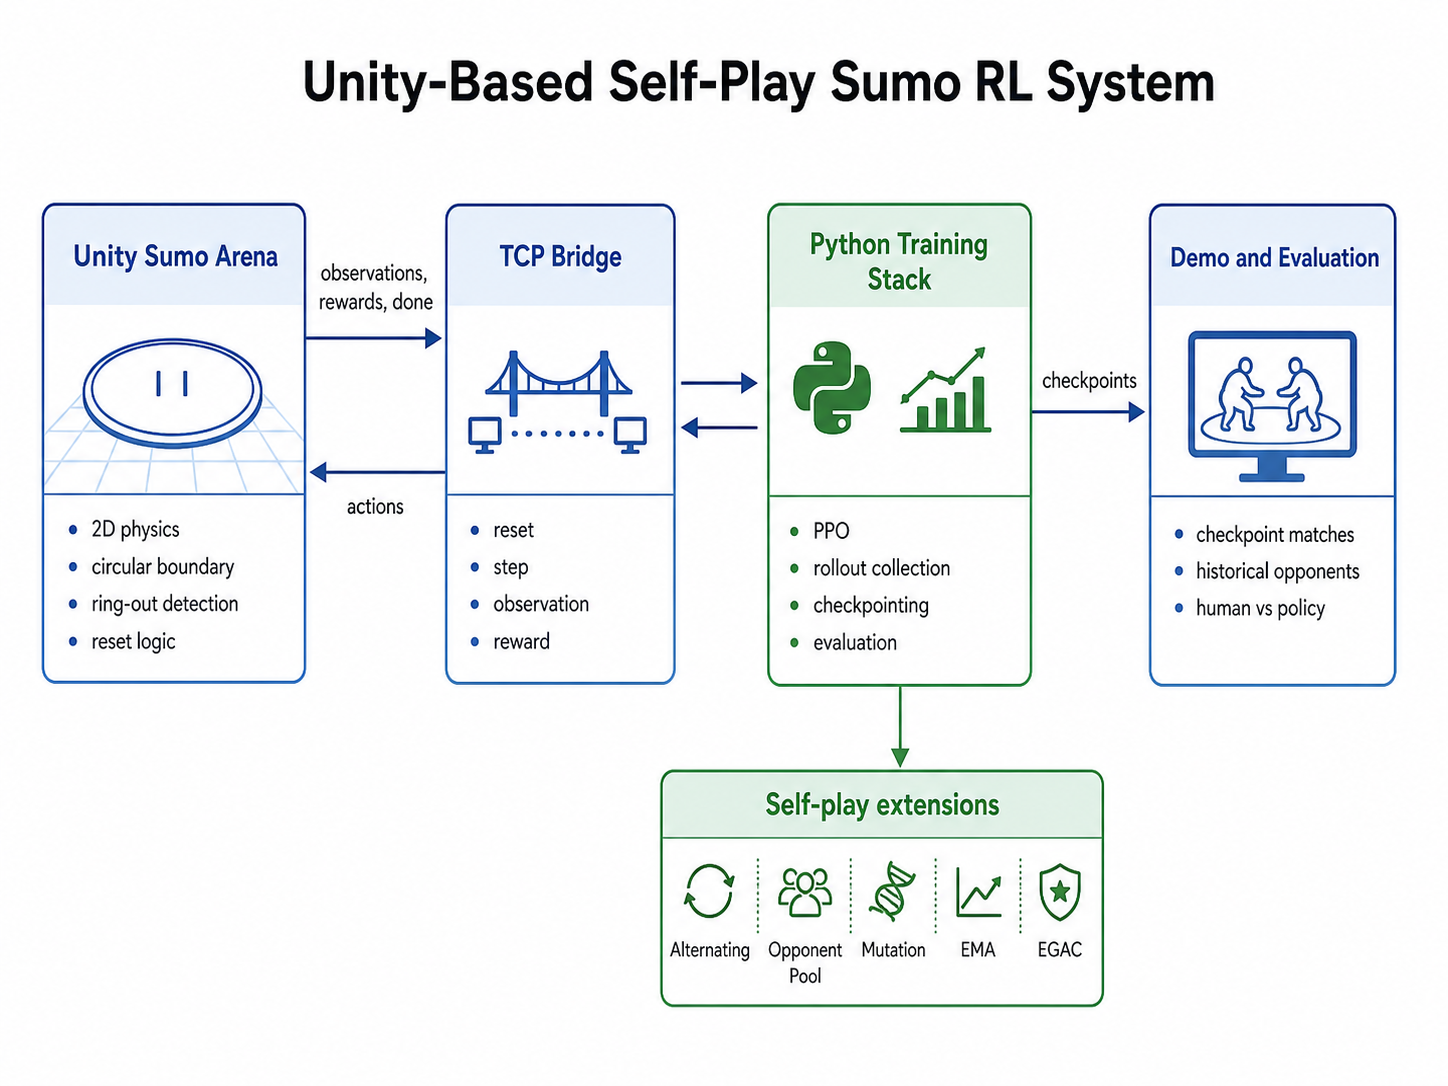
\includegraphics[width=\linewidth]{fig_system_overview.png}
    \caption{System overview. Unity handles the 2D sumo physics, boundary checks, reset logic, and demo scene. Python handles PPO training, self-play extensions, checkpoint management, and evaluation. A TCP bridge exchanges actions, observations, rewards, and terminal flags.}
    \label{fig:system}
\end{figure}

\section{Related Work}

Policy gradient methods are a standard foundation for continuous-control reinforcement learning. Proximal Policy Optimization (PPO) \citep{schulman2017ppo} is widely used because it combines a simple implementation with reasonably stable updates through a clipped surrogate objective. Generalized Advantage Estimation (GAE) \citep{schulman2016gae} further reduces variance by using a tunable bias-variance tradeoff for advantage computation. This project uses PPO as the baseline because it is practical for a small custom environment and easy to extend with self-play mechanisms.

Self-play has a long history in game-playing agents. AlphaGo Zero showed that self-play can produce superhuman behavior without human demonstrations in a perfect-information board game \citep{silver2017alphagozero}. Large-scale systems such as OpenAI Five extended self-play to complex team games with large compute budgets \citep{berner2019dota}. Smaller multi-agent environments have also demonstrated that competition can lead to emergent strategies and increasingly complex behavior \citep{bansal2018emergent}. Game-theoretic approaches such as Policy-Space Response Oracles (PSRO) provide a more formal population-based view of opponent selection \citep{lanctot2017psro}. The current project is much smaller, but it faces the same basic issue: latest-vs-latest self-play can be unstable and overly narrow.

Safety and constraint-aware reinforcement learning study how agents can satisfy behavioral restrictions while optimizing reward. Constrained Policy Optimization \citep{achiam2017cpo} is one principled approach, while broader surveys describe the challenge of avoiding unsafe exploration and unsafe actions \citep{garcia2015safe}. EGAC is not a full constrained RL method. Instead, it is a lightweight architectural bias: it uses known geometry of the arena to bias the actor away from high-risk boundary actions. This is closer in spirit to using domain structure to shape an action distribution than to solving a constrained optimization problem.

\section{Environment and System Design}

\subsection{Unity sumo arena}

The environment is a symmetric two-player arena. Each agent is represented by a 2D rigidbody. The arena is circular, and a ring-out occurs when an agent's position leaves the valid radius. The agents have no health bars, inventory, or complex abilities. The core interaction is movement and positional pressure: an agent tries to force the opponent closer to the boundary while avoiding its own ring-out.

Each agent has two high-level actions. The first is continuous movement in the plane. The second is a push or dash action triggered by a binary flag. Push has a cooldown, which prevents the optimal behavior from becoming continuous spamming. The push direction follows the agent's velocity direction. This choice makes the action interface compact for a learned policy: the actor outputs a movement vector and a push trigger, while the motor logic converts motion into physical impulse.

The Unity side contains separate components for agent motion, boundary checking, match control, batched arena stepping, and bridge communication. Manual physics simulation is used for training so that Python can send an action and receive the next state in a deterministic step-like loop. A real-time mode is also supported for human-vs-policy demonstration, where the human controls one agent with keyboard input and Python drives the other agent from a checkpoint.

\subsection{Python-Unity bridge}

The training stack communicates with Unity through a persistent TCP bridge. Python sends JSON commands such as \texttt{reset}, \texttt{step}, \texttt{reset\_batch}, and \texttt{step\_batch}. Unity responds with observations, rewards, terminal flags, winner information, and diagnostic status. A file bridge also exists as an early integration fallback, but the TCP bridge is the primary training path.

The Python side wraps this bridge in environment classes with familiar \texttt{reset}/\texttt{step}/\texttt{close} semantics. The single-arena wrapper is useful for debugging, rollout collection, and visible stepping. The vectorized wrapper supports batched arena instances, which improves sample throughput and exposes PPO updates to a broader set of episodes.

\subsection{Observation and action spaces}

The current observation vector has 17 dimensions. It includes the agent's own position and velocity, the opponent's position and velocity, relative position and velocity, explicit boundary features, and a push-ready flag. The boundary features are important because early versions of the policy often failed to reason about proximity to the edge. The relevant terms are self distance to center, self edge margin, opponent distance to center, and opponent edge margin.

The action vector has three dimensions:
\[
    a = (\text{move}_x, \text{move}_y, \text{use\_push}).
\]
The first two dimensions are continuous movement components, while the final dimension is interpreted as a Bernoulli push trigger. The action adapter converts this vector into the dictionary format consumed by Unity. Left-right canonicalization is applied to reduce redundant learning in mirrored spawn configurations.

\section{PPO Baseline}

The baseline policy is an actor-critic network with a small multilayer perceptron trunk. Given an observation vector $o_t$, the network produces a movement mean $\mu_t \in [-1,1]^2$, a push logit $\ell_t$, and a scalar value prediction $V(o_t)$. Movement is sampled from a diagonal Gaussian distribution and clipped to the valid range. The push decision is sampled from a Bernoulli distribution parameterized by the push logit.

PPO optimizes a clipped surrogate objective \citep{schulman2017ppo}. Let $\pi_\theta$ be the current policy, $\pi_{\theta_{\mathrm{old}}}$ be the policy used to collect trajectories, and
\[
    r_t(\theta)=\frac{\pi_\theta(a_t|o_t)}{\pi_{\theta_{\mathrm{old}}}(a_t|o_t)}.
\]
The clipped policy loss is
\[
    L^{\mathrm{clip}}(\theta) =
    \mathbb{E}_t\left[
    \min \left(
        r_t(\theta)\hat{A}_t,
        \mathrm{clip}(r_t(\theta), 1-\epsilon, 1+\epsilon)\hat{A}_t
    \right)
    \right].
\]
The implementation combines this policy term with a value loss and an entropy bonus:
\[
    L = -L^{\mathrm{clip}} + c_v L^V - c_e H(\pi_\theta).
\]
Advantages are computed using GAE \citep{schulman2016gae}. The baseline training loop collects steps from Unity, stores observations, actions, log probabilities, values, rewards, and done flags, computes returns and advantages, and then runs several epochs of minibatch PPO updates.

Plain PPO provides a useful starting point but is not sufficient for the final project goal. In the Unity sumo arena, a policy may learn high-variance behavior, overuse push, or fail to preserve safe distance from the edge. These problems motivated the self-play extensions and EGAC described below.

\section{Self-Play Stabilization Methods}

\begin{figure}[t]
    \centering
    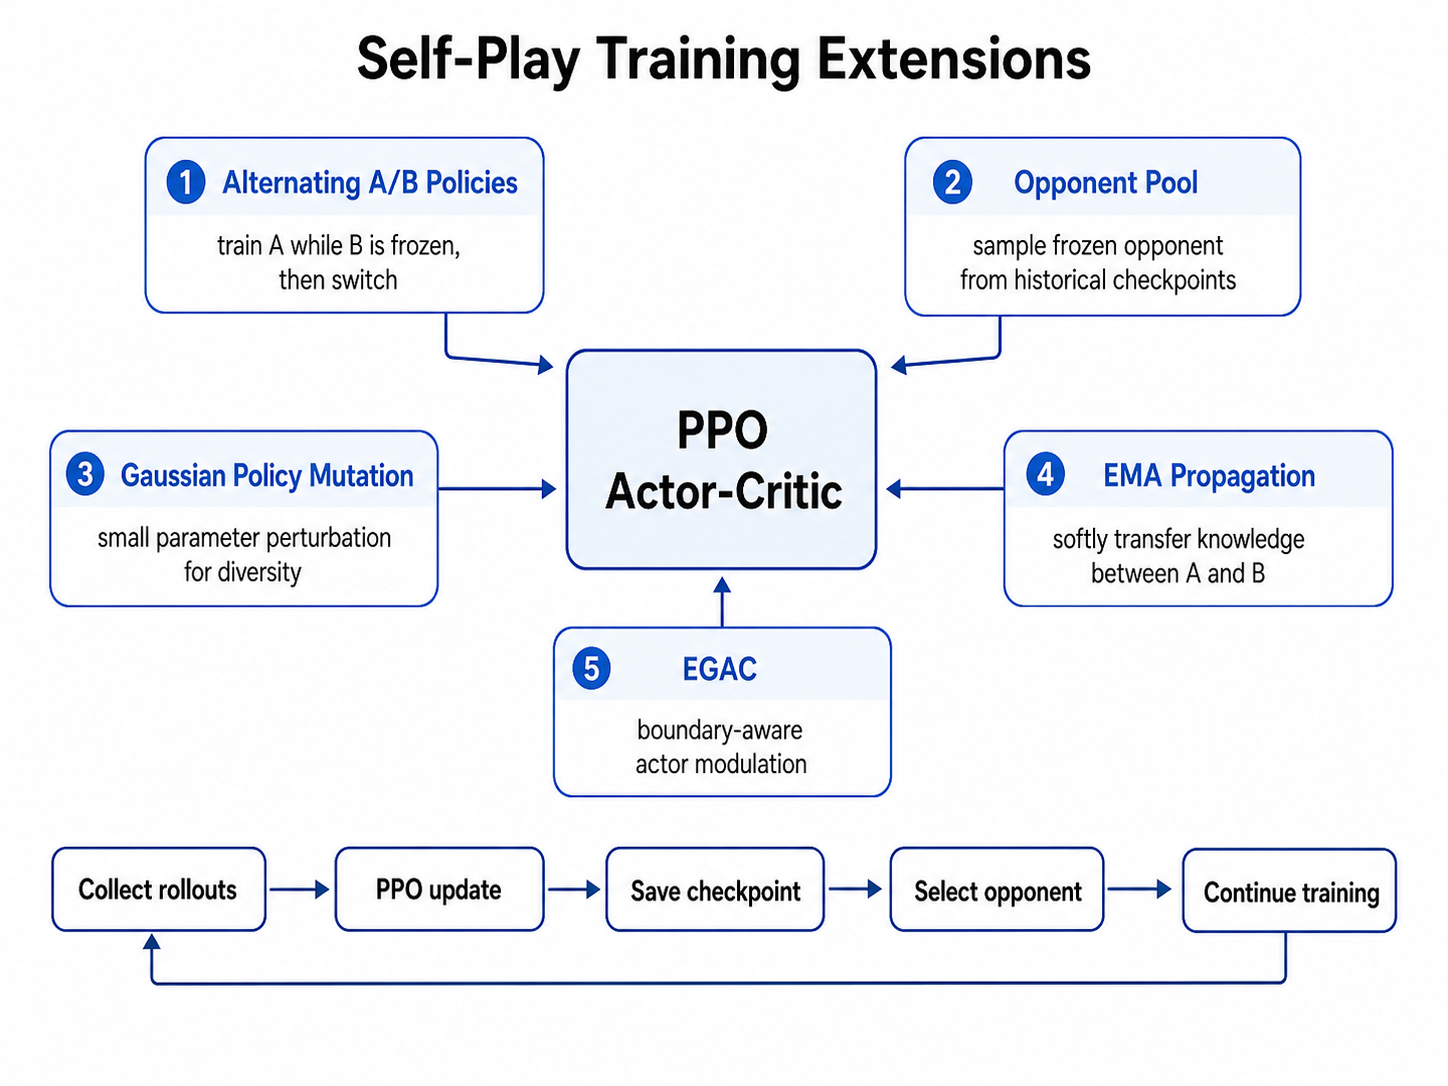
\includegraphics[width=\linewidth]{fig_training_pipeline_extensions.png}
    \caption{Training extensions on top of PPO. The implementation supports alternating two-policy self-play, opponent-pool sampling, Gaussian checkpoint mutation, EMA propagation, and EGAC. These extensions target different sources of brittleness in self-play.}
    \label{fig:extensions}
\end{figure}

\subsection{Alternating two-policy self-play}

A simple shared-policy self-play setup trains one policy against itself. This is attractive because the game is symmetric, but it can also produce synchronized failure modes. If both sides share the same mistaken behavior, the training signal may not clearly identify the weakness. For example, two identical policies may both overcommit near the boundary or both fail to punish obvious positional mistakes.

The implementation therefore supports alternating two-policy self-play. Two policies, $A$ and $B$, are maintained. During an $A$ segment, policy $A$ is updated while policy $B$ is frozen as the opponent. During the next segment, policy $B$ is updated while policy $A$ is frozen. This creates a clearer opponent distribution for each update segment and avoids changing both policies at the same instant.

The code also supports draining active episodes before a segment exits. This matters because switching sides in the middle of active matches can mix trajectories from different training regimes. Draining keeps segment boundaries cleaner and makes checkpoint comparisons easier to interpret.

\subsection{Opponent-pool sampling}

Latest-vs-latest self-play can overfit to the most recent opponent. A policy may become strong against its current counterpart while forgetting how to handle older or qualitatively different policies. To reduce this narrowness, the training entry point maintains a pool of historical two-policy checkpoints. Before a new training segment, the frozen opponent side can be replaced by the corresponding side from a sampled historical checkpoint.

This mechanism is simpler than a full league or PSRO system \citep{lanctot2017psro}, but it addresses the same high-level issue: the current learner should face a distribution of opponents rather than a single latest opponent. In this project, the opponent pool is especially useful for final evaluation because it naturally creates historical policies to test against.

\subsection{Gaussian policy mutation}

Self-play can converge to local conventions. If both policies adapt to the same weak behavior, additional exploration may be needed to escape. The project includes Gaussian checkpoint mutation as a lightweight diversity mechanism. At selected segment boundaries, the parameters of the side about to train are perturbed:
\[
    \theta' = \theta + \sigma \epsilon,\quad \epsilon \sim \mathcal{N}(0,I).
\]
The mutation standard deviation controls the strength of the perturbation. Small values preserve most learned behavior while nudging the policy into nearby alternatives. Large values risk destroying useful structure. In the report, this method should be understood as Gaussian policy mutation or checkpoint perturbation, not image-style Gaussian blur.

\subsection{EMA propagation}

Alternating self-play separates the two policies, but complete separation can also be undesirable. One side may improve while the other remains stale, causing the training process to oscillate. To smooth this process, the implementation can apply exponential moving average propagation after a side finishes training:
\[
    \theta_{\mathrm{target}} \leftarrow
    \alpha \theta_{\mathrm{target}} + (1-\alpha)\theta_{\mathrm{source}}.
\]
Here the source is the newly trained side, and the target is the opposite side. EMA propagation softly transfers useful behavior without directly copying the entire policy. It is intended to preserve diversity while reducing extreme divergence between $A$ and $B$.

\subsection{Reward and observation shaping}

The project also uses environment-specific reward and observation shaping. Sparse win/loss rewards are clean, but they can be weak in a physical arena where many steps occur before terminal feedback. The implemented shaping terms include edge-safety penalties, outward-pressure rewards, time-scaled terminal loss penalties, and timeout center-bias penalties. These terms are not meant to replace winning as the objective. Instead, they provide intermediate signals for behaviors that are strongly related to success: staying away from the edge, pushing the opponent outward, and avoiding passive timeout behavior.

Observation shaping is equally important. The current 17-dimensional observation vector includes explicit edge features, which are later reused by EGAC. Without these features, the policy must infer boundary risk indirectly from coordinates. With them, both the reward function and the actor architecture can reason more directly about ring-out risk.

\section{Edge-Gated Actor-Critic}

\begin{figure}[t]
    \centering
    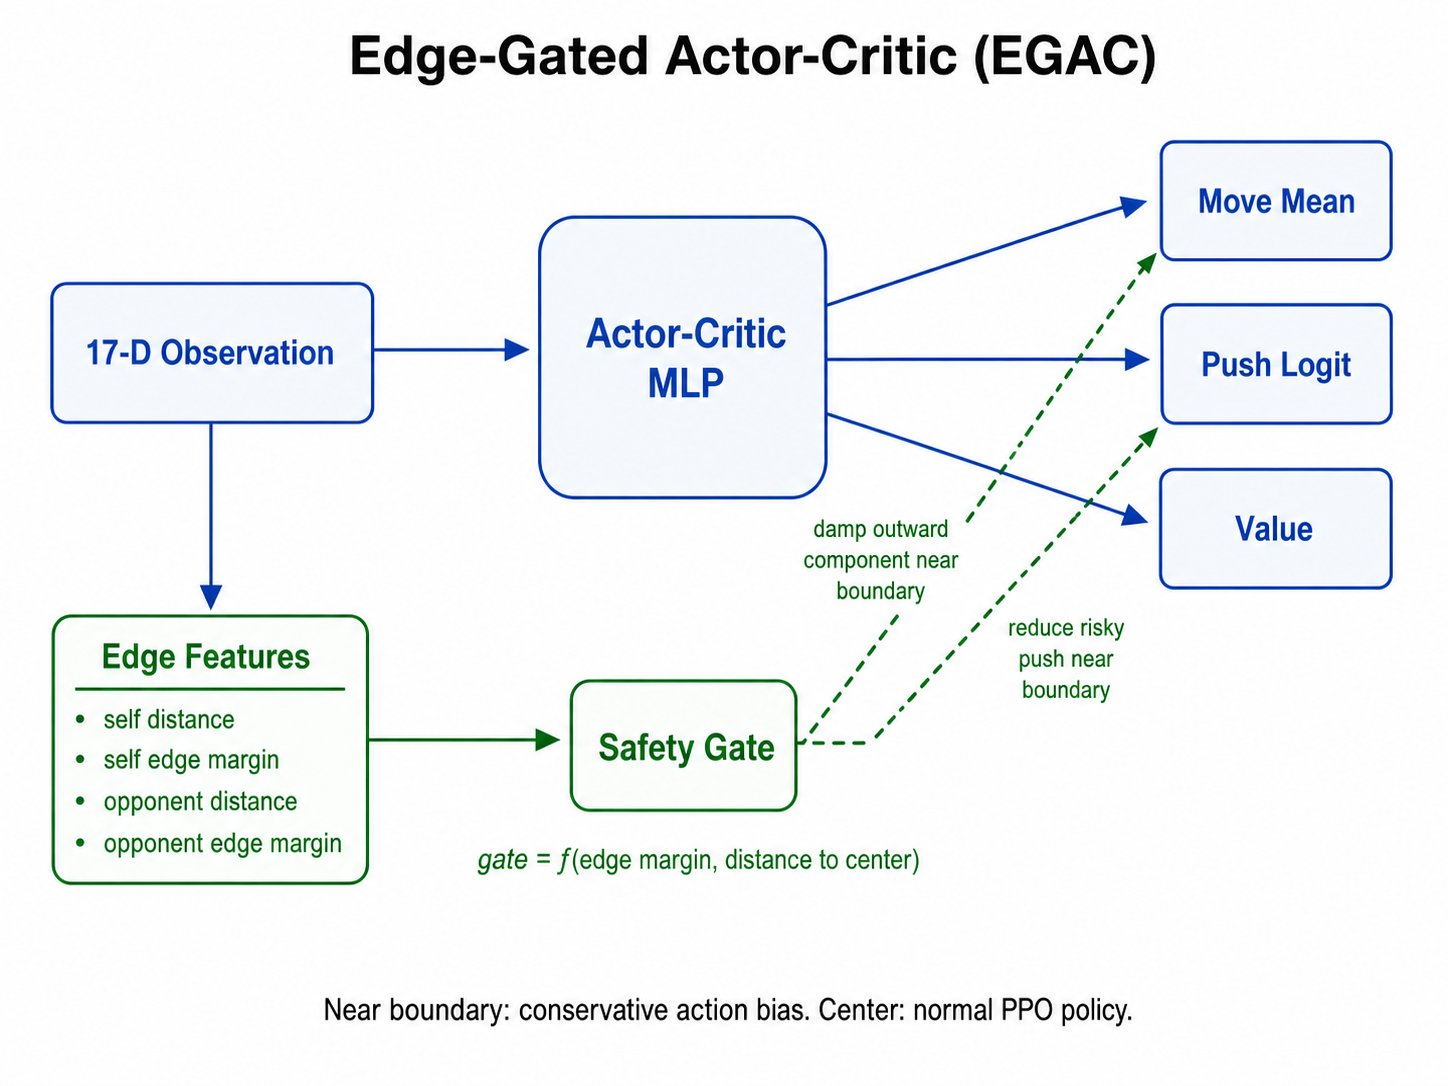
\includegraphics[width=\linewidth]{fig_egac_architecture.png}
    \caption{Edge-Gated Actor-Critic. EGAC reuses boundary features from the observation vector to generate a safety gate. The gate dampens outward movement near the boundary and penalizes risky push logits while leaving inward recovery movement available.}
    \label{fig:egac}
\end{figure}

\subsection{Motivation}

In a plain MLP actor, all observation features are mixed into one latent representation. The same network must learn when to attack, when to recover, and when push is dangerous. In the sumo arena, the cost of a wrong action depends strongly on boundary geometry. A push near the center may be useful, while the same push near the edge may cause self ring-out. This creates a natural opportunity for an architectural bias: the actor should become more conservative when the agent is near the boundary, but it should not become passive everywhere.

EGAC implements this bias directly in the actor. It does not change the Unity environment or the PPO loss. Instead, it changes how the policy distribution is parameterized. The actor still outputs a movement mean and push logit, but a boundary-aware gate modulates these outputs before sampling.

\subsection{Architecture}

Let $p \in \mathbb{R}^2$ be the self position in arena coordinates, and let $r = p / \|p\|$ be the outward radial direction. Let $\mu$ be the raw movement mean predicted by the actor. The outward component of $\mu$ is
\[
    \mu_{\mathrm{out}} = \max(0, \mu^\top r)r.
\]
EGAC computes a safety gate $g \in [g_{\min},1]$ from edge-related features. In the implementation these include self distance to center, self edge margin, opponent distance to center, and opponent edge margin. A simple learned gate is combined with a deterministic boundary-safety term derived from the self edge margin.

The final movement mean is
\[
    \mu' = \mu - (1-g)\mu_{\mathrm{out}}.
\]
Thus, when the agent is near the boundary and $g$ is small, outward motion is damped. Inward motion is not removed, which allows the agent to recover toward the center. The push logit is also modified:
\[
    \ell'_{\mathrm{push}} =
    \ell_{\mathrm{push}} - \lambda(1-g).
\]
The coefficient $\lambda$ controls how strongly near-edge risk suppresses push probability.

\begin{figure}[t]
    \centering
    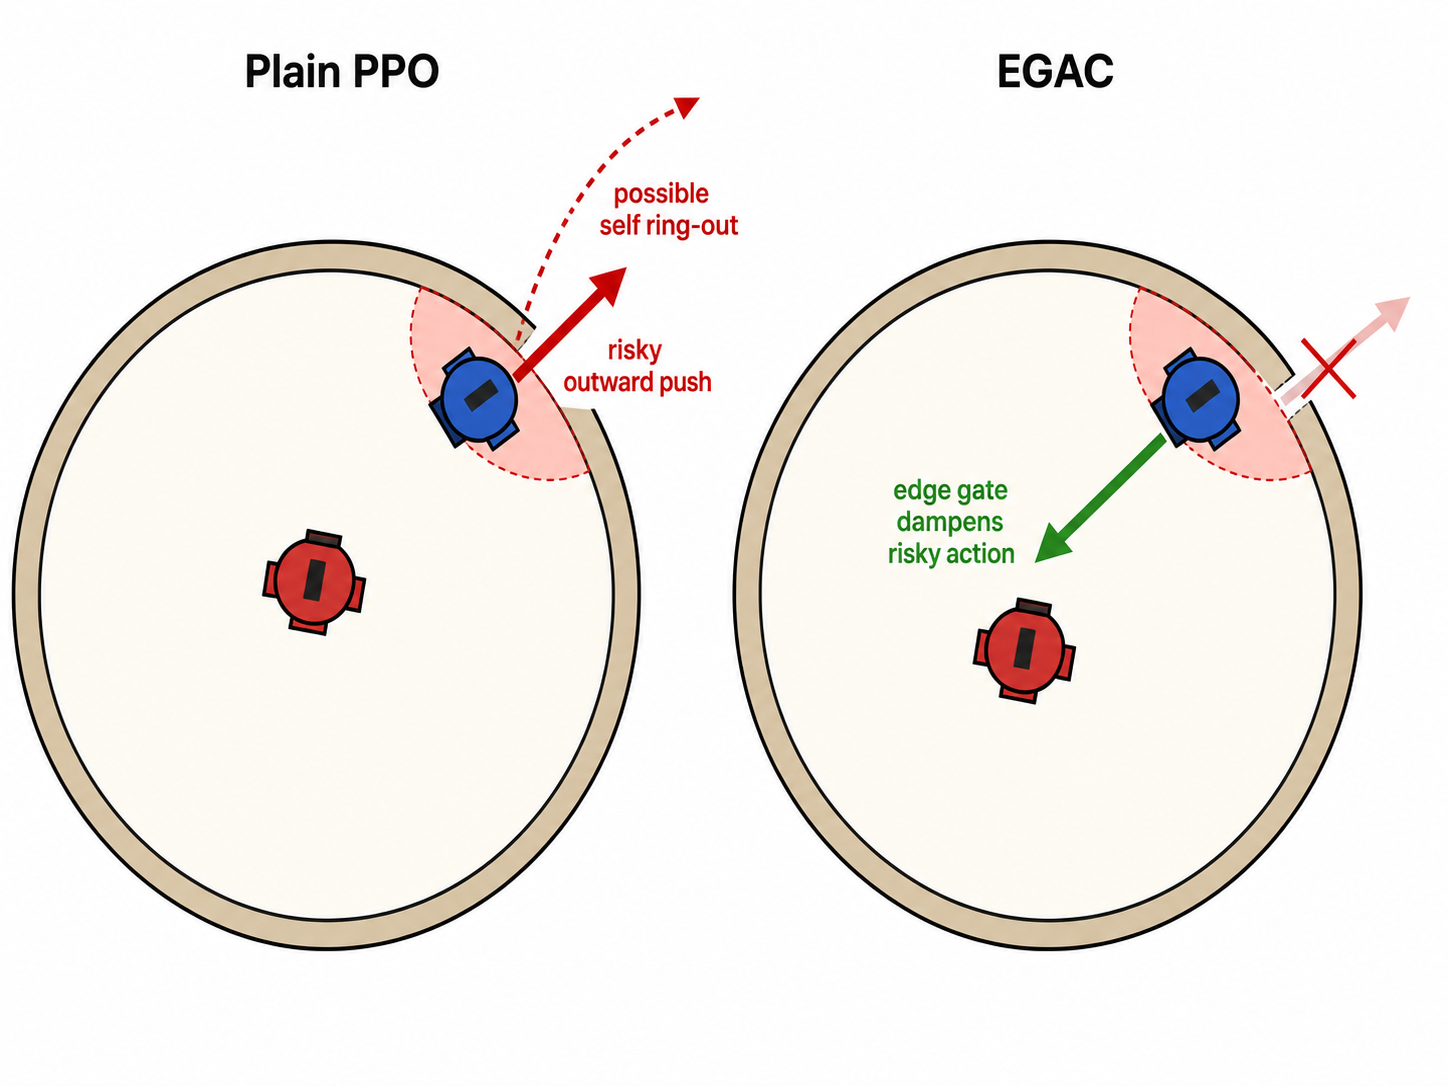
\includegraphics[width=\linewidth]{fig_behavior_comparison.png}
    \caption{Qualitative behavior targeted by EGAC. Plain PPO may output risky outward movement or push near the boundary. EGAC biases the actor toward safer recovery actions when edge risk is high.}
    \label{fig:behavior}
\end{figure}

\subsection{Difference from reward shaping}

EGAC is related to edge-aware reward shaping, but it operates at a different point in the learning system. Reward shaping changes the scalar feedback after an action has been taken. EGAC changes the policy's action distribution before the action is sampled. This means the model has a structural preference against high-risk boundary actions, while still learning from PPO updates.

This distinction is useful for the final project narrative. The reward terms teach the agent that boundary mistakes are costly. EGAC makes that lesson easier to express by giving the actor a specific mechanism for modulating aggression near the edge. The method remains lightweight: it adds a small gate head and a few deterministic operations, without requiring a new reinforcement learning algorithm.

\section{Evaluation Protocol and Ablation Design}

\begin{figure}[t]
    \centering
    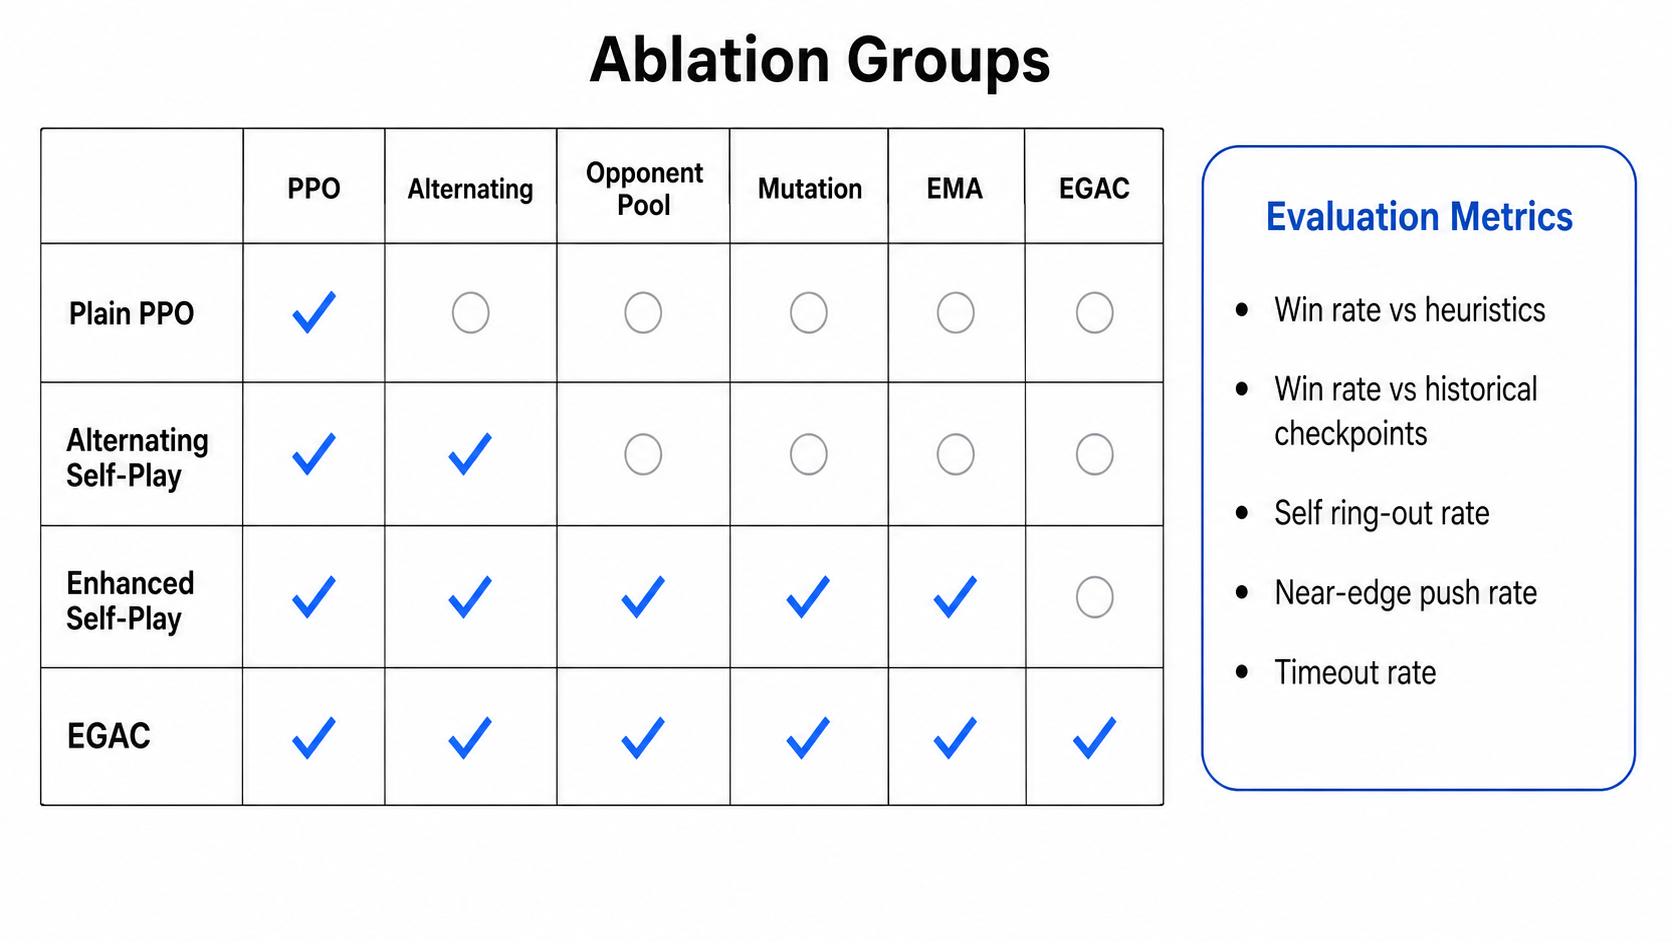
\includegraphics[width=\linewidth]{fig_ablation_design.png}
    \caption{Ablation design. The report separates plain PPO, alternating self-play, enhanced self-play, and EGAC. This design isolates the contribution of the proposed edge-gated actor from other self-play stabilization methods.}
    \label{fig:ablation}
\end{figure}

The final deadline did not leave enough time for a complete large-scale ablation. Instead, the project defines a concrete evaluation protocol that can be run with the implemented code. This protocol is important because a single training reward curve is not sufficient to judge self-play quality. A policy can improve against the latest opponent while becoming worse against older opponents or more brittle against humans.

\subsection{Ablation groups}

The planned ablation contains four main groups. Plain PPO uses the base actor-critic without self-play extensions. Alternating self-play adds A/B policy switching and the shaped observation/reward setup. Enhanced self-play adds opponent-pool sampling, Gaussian policy mutation, and EMA propagation. EGAC adds the boundary-aware actor gate on top of the enhanced setting.

\begin{table}[t]
    \centering
    \caption{Method components used in the ablation design.}
    \label{tab:components}
    \begin{tabular}{lccccc}
        \toprule
        Method & Alternating & Pool & Mutation & EMA & EGAC \\
        \midrule
        Plain PPO & -- & -- & -- & -- & -- \\
        Alternating Self-Play & \checkmark & -- & -- & -- & -- \\
        Enhanced Self-Play & \checkmark & \checkmark & \checkmark & \checkmark & -- \\
        EGAC & \checkmark & \checkmark & \checkmark & \checkmark & \checkmark \\
        \bottomrule
    \end{tabular}
\end{table}

\subsection{Metrics}

The most important metrics are behavioral rather than only reward-based. Win rate against heuristic opponents measures basic competence outside the self-play loop. Win rate against historical checkpoints measures robustness to a broader opponent distribution. Self ring-out rate measures how often the evaluated agent loses by leaving the boundary. Near-edge push rate measures the frequency of push actions when edge margin is below a threshold. Timeout rate checks whether safer behavior comes from excessive passivity. Mean episode length provides additional context about whether the policy is failing immediately, engaging productively, or stalling.

For EGAC, the primary expected effect is not necessarily a large immediate reward increase. The more direct hypothesis is that EGAC should reduce self ring-outs and near-edge push actions while preserving the ability to engage near the center. If timeout rate rises sharply, that would indicate that the gate made the policy too conservative. If near-edge push rate decreases without a large timeout increase, the gate is behaving as intended.

\subsection{Qualitative analysis}

Visual inspection is a strength of this project. Unity makes it possible to observe whether a policy is actually controlling space or simply surviving by chance. The human-vs-policy mode also provides a useful stress test: a brittle policy can often be baited into self ring-out by a human player, while a more robust policy should recover inward near the boundary.

The qualitative comparison in Figure~\ref{fig:behavior} illustrates the failure mode targeted by EGAC. It should be paired with a Unity screenshot or short video in the final presentation. In a complete evaluation, the same checkpoint should be tested with and without EGAC disabled only if the architectures are comparable; otherwise, the cleaner comparison is between separately trained enhanced self-play and EGAC policies.

\section{Implementation Details}

The Python training code is organized around modules for environments, agents, algorithms, and evaluation scripts. The environment wrappers communicate with Unity through the TCP client. Observation and action adapters keep the training-facing vectors separate from the JSON bridge format. PPO training is implemented in a dedicated trainer with configurable update count, rollout length, minibatch size, learning rate, entropy coefficient, reward shaping terms, and self-play mode.

The default training configuration uses batched Unity arenas when available. Each arena can reset with a derived seed so that spawn side swaps and jitter are reproducible. Checkpoints store either a single policy or a two-policy pair. The alternating self-play entry point can continue from an existing checkpoint, sample an opponent from the pool, apply mutation, run a training segment, save the result, and optionally apply EMA propagation.

EGAC is controlled by configuration flags. When \texttt{use\_edge\_gate} is false, the actor behaves as the original MLP actor-critic. When it is true, the actor creates a small gate head over edge features and applies movement/push modulation in the forward pass. The main parameters are \texttt{edge\_gate\_margin}, \texttt{edge\_gate\_min\_safety}, \texttt{edge\_gate\_push\_penalty}, and \texttt{edge\_gate\_hidden\_size}. The human-vs-policy script also reconstructs the correct actor architecture from checkpoint configuration, so EGAC policies can be demonstrated in real time.

The Unity implementation includes two training modes. In manual simulation mode, each Python step advances Unity physics by a fixed duration. This is used for PPO training and batch stepping. In real-time mode, Unity physics runs normally and Python repeatedly sends the latest action for the external agent. This separation avoids mixing training-time deterministic stepping with presentation-time interactive control.

\section{Discussion}

The project's main achievement is an operational full-stack self-play system. Building a custom Unity environment and connecting it to Python training code required solving several practical problems before algorithmic experiments became meaningful: stable bridge communication, reset behavior, action conversion, observation vectorization, checkpoint compatibility, batched stepping, and real-time demo control. Once these components were in place, the project could focus on learning behavior.

The self-play extensions address different failure modes. Alternating policies reduce shared-policy synchronization. Opponent pools reduce latest-opponent overfitting. Gaussian mutation increases local diversity. EMA propagation smooths knowledge transfer between A and B. Reward shaping and observation engineering expose boundary risk to the learner. EGAC then uses that boundary information as an architectural bias. The combination is not a complete league training system, but it is a coherent set of mechanisms for a small course project.

There are also limitations. The final code is better described as an experimental framework than a polished benchmark suite. The project does not yet include a full statistical comparison over many seeds. The opponent pool is lightweight and does not implement game-theoretic meta-strategy selection. Gaussian mutation is simple and may be sensitive to its standard deviation. EGAC may reduce risky behavior but could also make policies overly conservative if the push penalty is too strong. These limitations motivate the evaluation protocol described above.

Future work would include running the ablation over multiple seeds, adding automated metric logging for near-edge push rate, exporting policies for direct Unity inference, and comparing EGAC to explicit action shielding. Another direction is to learn a separate risk critic that predicts self ring-out probability, then use it either as an auxiliary loss or as a more adaptive gate. A larger population-based method could also replace the current opponent pool.

\section{Conclusion}

This project built a Unity-based self-play reinforcement learning system for a two-agent sumo arena. The environment is intentionally simple, but it exposes meaningful challenges: sparse terminal feedback, unstable self-play, overfitting to the latest opponent, and high-risk boundary behavior. The implementation supports PPO training, alternating two-policy self-play, opponent-pool sampling, Gaussian mutation, EMA propagation, shaped rewards, batched arenas, checkpoint evaluation, and human-vs-policy demonstration.

The proposed EGAC architecture adds a project-specific contribution by injecting boundary risk into the actor. By damping outward movement and reducing push probability near the boundary, EGAC targets one of the most visible failure modes in the arena: self ring-out caused by aggressive actions at the edge. The result is a compact platform for studying how small architectural biases and self-play training mechanisms affect behavior in a physical competitive environment.

\bibliographystyle{plainnat}
\bibliography{references}

\end{document}
